\documentclass[10pt, a4paper]{article}

\usepackage{geometry}
\geometry{includeheadfoot,textheight=26cm,textwidth=18cm}
\usepackage{amsthm,amsmath,natbib}
\usepackage{latexsym, amsfonts, amssymb, amscd}
\usepackage{bbm}
\usepackage{graphicx}
\usepackage{subfigure}

\usepackage{titlesec}
\titlespacing*{\section}{0pt}{0.5ex plus .2ex minus .2ex}{0.5ex plus .2ex}[0pt]

\usepackage{titling}
\setlength{\droptitle}{-3cm}
\renewcommand{\maketitlehookd}{\vspace{-1cm}}

\title{Hierarchical Tractography Optimisation}
\date{}
\author{
Matteo Frigo$^{3,1,2,\dagger}$, Muhamed Barakovic$^{1}$, Jean-Philippe Thiran$^{1}$, Alessandro Daducci$^{1,2}$\\
$^{1}$Signal Processing Laboratory LTS5, EPFL, Switzerland,\\ $^{2}$Computer Science Department, University of Verona, Italy\\ $^{3}$Universit\'{e} C\^{o}te d'Azur, Inria, France\\
$^{\dagger}$matteo.frigo@inria.fr
}

\begin{document}
\maketitle
\section{Introduction}In this work we tackle the recently identified bias related to the presence of many false positive connections within connectomes. This fact has been addressed in a recent work of Maier-Hein et al. \cite{meierhein}, where the authors analised the result of 96 the tractography pipelines submitted at the ISMRM2015 tractography challenge. They showed how \emph{most algorithms routinely extracted many false positive bundles}, concluding that \emph{tractography identifies more invalid than valid bundles}. The balancing of sensitivity and specificity of the connectomes resulting from tractography has been studied by Zalesky et al. \cite{zalesky} and Thomas et al. \cite{thomas}. What they concluded is that \emph{specificity is at least twice as important as sensitivity} and that \emph{the methods that show the highest sensitivity show the lowest specificity, and viceversa}. The solution will be formulated as a convex optimisation problem that simultaneously fits the acquired data and promotes sparsity with an hierarchical pattern.

\section{Methods}What we propose is a method that takes a tractogram as input and detects the tracks corresponding to false positive connections among those provided. The data fitting is treated in the same way as COMMIT does. First introduced by Daducci et al. \cite{daducci}, this tool defines a dictionary that describes a tractogram through a microstructure model (in our case Ball \& Stick), then it looks for the linear combination of its atoms that best fits (in NNLS sense) an acquired signal or an anatomical map (in our case NODDI). Finally the fibres associated to null coefficients will be false positive elements. Moreover, the connections between different regions of the brain cortex are endowed with a hidden hierarchical pattern. We model this knowledge by considering a tree structured graph of the connections, motivated by the fact that most tractography algorithms are designed in such a way that there are multiple paths between two points of the cortex and duplicates are a natural consequence of using seeding-based algorithms. We want that the property \emph{being a false positive} propagates from anchestor to child in the tree graph described before, hence we penalise the data fitting term with the hierarchical sparsity term described in equation \eqref{omega} and analysed in \cite{jenatton}. We call our method \emph{Hierarchical Non-Negative Least Squares} (HNNLS) in analogy with NNLS.
\begin{equation}
\label{omega} \Omega(x) = \sum_{g\in\mathcal{G}}\|x_{|g}\|_2
\end{equation}

\section{Results}We worked on the ISMRM2015 challenge dataset, which is endowed with 25 valid bundles (VB) and 785 invalid bundles (IB). The ideal result preserves 25 VB and 0 IB. Two state-of-the-art algorithms for tractography optimisation have been chosen as benchmark: SIFT2 and LiFE. Our model outperforms these methods showing that the intrinsic hierarchical structure that characterises both the anatomy of the brain and the result of tractography algorithms can be exploited in the task of detecting the false-positive connections within connectomes.

\begin{center}
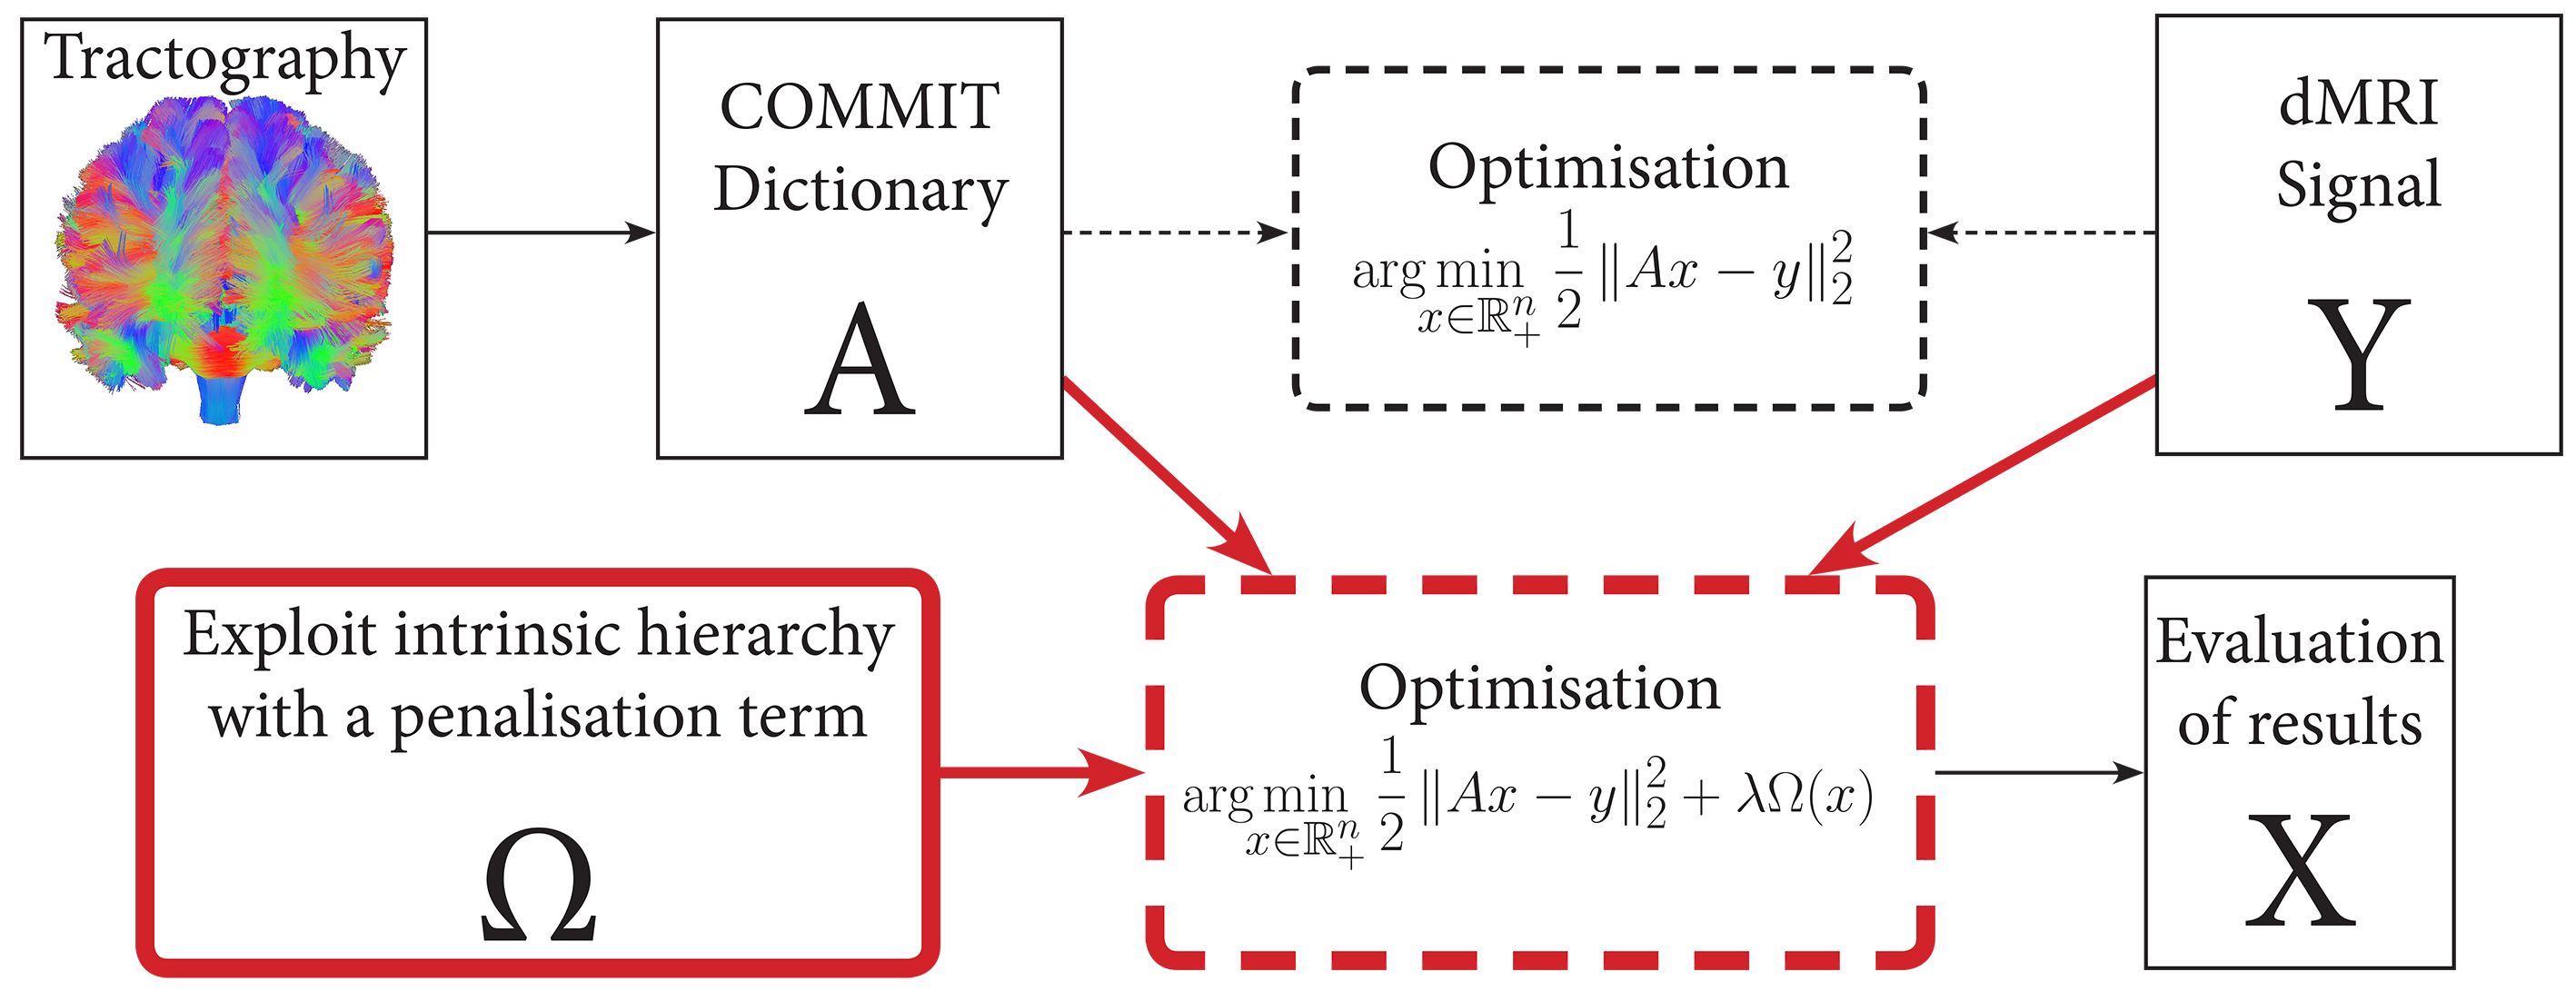
\includegraphics[width=.5\textwidth]{diagram}
\qquad
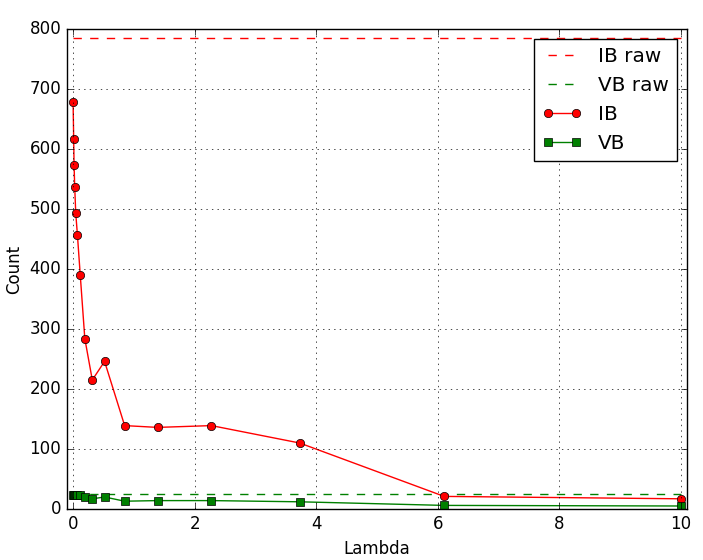
\includegraphics[width=.24\textwidth]{results}
\end{center}



\bibliographystyle{alpha}
\begin{thebibliography}{}
\bibitem{meierhein}
Maier-Hein, et al.
\newblock {\em Tractography-based connectomes are dominated by false-positive connections,} biorxiv, 2016.

\bibitem{zalesky}
Zalesky et al.
\newblock {\em Connectome sensitivity or specificity: which is more important?,} Neuroimage, 2016.

\bibitem{thomas}
Thomas et al.
\newblock {\em Anatomical accuracy of brain connections derived from diffusion MRI tractography is inherently limited,} Proceedings of the National Academy of Science, 2014.

\bibitem{daducci}
Daducci et al.
\newblock {\em COMMIT: convex optimization modeling for microstructure informed tractography.,} IEEE Transactions on Medical Imaging 2015.

\bibitem{jenatton}
Jenatton, Rodolphe, et al.
\newblock {\em Proximal methods for hierarchical sparse coding,} Journal of Machine Learning Research, 2011.

\end{thebibliography}

\end{document}
